\documentclass[10pt,conference,compsocconf]{IEEEtran}

\usepackage{hyperref}
\usepackage{graphicx}	% For figure environment

\begin{document}
	\title{Project 1 - To the pursuit of the Higgs Boson}
	
	\author{
		L\'ea Bommottet, Nicolas Brunner, Karine Perrard\\
		\textit{ EPFL, Switzerland}
	}
	
	\maketitle
	
	\section{Introduction}
	
	Sexy introduction about ML and the problem,
	we choose to have  with 4 different model in function of the data, and all the different models???  
	30 parameters
	
	\section{Models and methods}
	
	\subsection{Choice of Models}
	First of all, we have to select the core of our model. In this project, there is 6 possible models on which we can base.
	\subsubsection{Linear regression using gradient descent}
	
	This model try to minimize the error of the function, by moving the vector w in the reverse trajectory of the gradient.
	$$w^{(t+1)}=w^{(t)} -\gamma \nabla L(w^{(t)})$$
	$$e = y-Xw$$
	$$\nabla L(w) = -\frac{1}{N}X^te$$
	
	\subsubsection{Linear regression using stochastic gradient descent}
	
	The error function is defined as a sum over the training errors. \\
	$$ L(w) = \sum\limits_{n=1}^N L_n(w)$$
	As for gradient descent, we want to follow the gradient, but this time the updating step is done on the cost contributed by one of the training examples. We can also compute the gradient on a subset of the examples, this is mini-batch stochastic gradient descent.
	$$w^{(t+1)}=w^{(t)} -\gamma \nabla L_n(w^{(t)})$$
	
	
	\subsubsection{Least squares regression using normal equations}
	
	We try to solve: $\nabla L(w^*) = 0$
	
	Then we derive
	$$w^* = (X^\top X)^{-1}X^\top y$$
	and a unknown data-point would have 
	$$\hat y_m := x_m^\top w^*$$
	
	\subsubsection{Ridge regression using normal equations}
	
	We want to punish complex models and conversely choose simpler ones.
	In the case of ridge regression, we add a regularizer $\Omega(w) = \lambda||w||_2^2$ in the quest to minimize w:
	$$\min\limits_{w} L(w) + \Omega(w)$$
	the explicit solution of w become:
	$$w_{ridge}^* = (X^\top X+2N\lambda I)^{-1}X^\top y$$
	\subsubsection{Logistic regression using gradient descent or SGD}
	Add description + formulas
	\subsubsection{Regularized logistic regression using gradient descent or SGD}
	Add description + formulas
	
	
	The reason we based our model on ??? is because we have the least global error on the dataset. Fig.1 
	
	Furthermore, in function of the feature named "fit", some parameters are unavailable. Thanks to this important information, we don't train only one model, but 4, since "fit" can be {0,1,2,3}.
	This idea reduce our global error, when compared to an single model without this separation. Fig.2
	
	\subsection{Choice of parameters}
	Blablabla
	Cross-correlation by K-fold:
	
	As seen in Fig.3, the parameters that reduces most the train error are lambda = ??? and gamma = ???.
	
	\subsection{Choice of features}
	
	We can improve our model by adding new features, which are function of other parameters. We want more features that have a Normal distribution. 
	\begin{description}
		\item[Natural logarithm] \ \\
		Applying the logarithm on a parameter can highlight its Normal behavior. One example is this function on the feature 21 (Fig.~\ref{fig:feature21function}). In this case, we notice a much nicer Gaussian distribution on the values, than the initial data. By doing an exhaustive research, we find that the useful parameters with this function are [0, 1, 2, 3, 4, 5, 8, 9, 10, 13, 16, 19, 21, 23, 26, 29], when discarding the NaN value.
		\item[Square root] \ \\
		Same as the natural logarithm, the square root can bring out a normal distribution. The feature 21 is also transformed with this function in our model (Fig.~\ref{fig:feature21function}). Again if we don't consider the NaN value, the parameters [0, 13, 16, 21, 23, 26, 29] have a Normal behavior under the square root
		\item[Threshold] \ \\
		Add description + picture where a parameter is nice
		\item[Nothing max] \ \\
		Add description + picture where a parameter is nice
		\item[Nothing norm] \ \\
		Add description + picture where a parameter is nice
		\item[Distance] \ \\
		When we plot 2 parameters in a graph, we can find some correlation between (Fig.3). To reduces this property to a normal distribution, we compute the Manhattan distance. + picture where a parameter is nice
		\item[Nth power] \ \\
		Add description + picture where a parameter is nice
	\end{description}
	\section{Results}
	On compare entre model simple et le 4 jets.
	
	On montre les graph features, pourquoi certaines sont sqrt, del, cube.
	\begin{figure}[tbp]
		\centering
		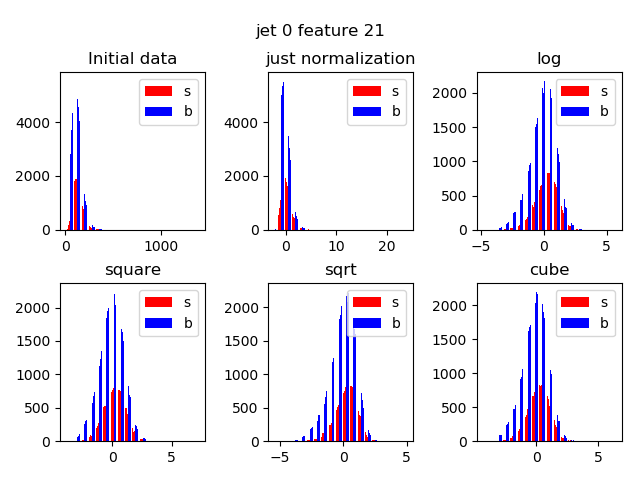
\includegraphics[width=\columnwidth]{21_0}
		\caption{Function applied on the data of the feature 21}
		\vspace{-3mm}
		\label{fig:feature21function}
	\end{figure}
	On compare avec et sans ces features en plus.
	
	On montre notre erreur global, on parle de kaggle?
	
	
	
	\section{Discussion}
	
	Separating our model into 4 different ones was a great idea, reducing considerably our global error (Fig.1) in the same way that including more parameters (Fig.2). Those added criterion improve the quality of our model, adjusting from ??? to ???.    
	
	
	
	\section{Summary}
	0.18\% of error is kinda ok with the simplicity of the core models. If we want to improve it more, we would need to find more useful parameters to boost our data.
	
	\section*{Acknowledgements}
	On est tous trop beau: et c'est pas nos r\'ef\'erence en dessous si jamais
	
	\bibliographystyle{IEEEtran}
	\bibliography{literature}
	
\end{document}
